\documentclass{report}

\usepackage{url}
\usepackage{cite}
\usepackage[version=4]{mhchem}
\usepackage{graphicx}
\usepackage{subfigure}
\usepackage[a4paper,top=2cm,bottom=2cm,right=3cm,left=3cm,marginparwidth=1.75cm]{geometry}


\title{3CL SARS-CoV-2 3CL Protease Analyzing}
\author{Yan Haoming}
\date{September 27, 2024}


\begin{document}
\maketitle
\begin{abstract}
    pass now.

\textbf{Keywords: }
\end{abstract}

\chapter{Protein Purification}
\section{\textit{E.coli} Lysis: Homogenizer}
\begin{itemize}
    \item Stir the buffer lysis containing \textit{E.coli} until without obvious lumps and precipitates in an ice bath.
    \item Filter the mixture (50 mL) by gauze and then pour into the \textbf{homogenizer}\cite{Homogenization} with 10 mL \ce{H2O} following the below settings:
    \begin{itemize}
        \item Raise the pressure to 1,000 bar for 2 minutes.
        \item Pause 1 minute.
        \item Repeat the cycle 3 times.
    \end{itemize}
    \item Centrifugate the liquid at 14,000 rpm for 30 minutes.
    \item Strain the product through a filter (0.45 $\mu$m) into a graduated cylinder.
\end{itemize}
\section{Purification: Column Chromatography}
\subsection{Affinity Chromatography: Immobilized \ce{Ni^2+} Metal Ion + His-tag}
\subsection{Gel-filtration Chromatography}
\section{Analyzing: SDS-PAGE}

\chapter{Enzyme Kinetics}
\begin{figure}
    \centering
    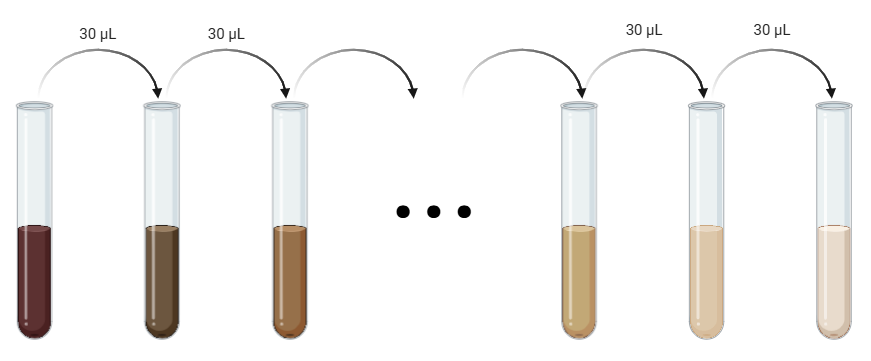
\includegraphics[width=0.7\linewidth]{../Figures/serial dilution.png}
    \caption{Serial Dilution of Inhibitor}
    \label{Serial Dilution of Inhibitor}
\end{figure}
\begin{figure}
    \centering
    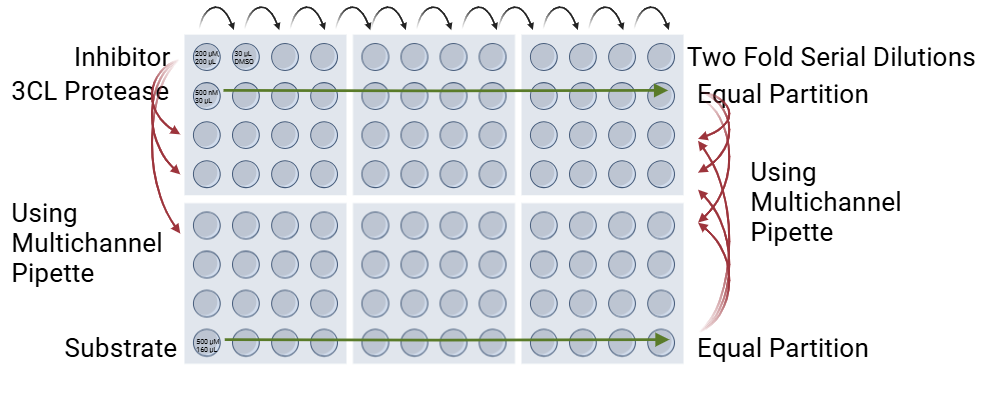
\includegraphics[width=1\linewidth]{../Figures/microplate.png}
    \caption{Solution Configuration in Microplate}
    \label{Inhibitor Solution Configuration in Microplate}
\end{figure}
The following experiments involve tedious configuration of solutions with different concentrations, including substrate, 3CL Protease (Enzyme), and inhibitor.
To summarize and visualize the complicated process of dilution, I have drawn the Figure \ref{Inhibitor Solution Configuration in Microplate}.
Generally speaking, we used \textbf{multichannel pipette} to transfer a whole row of solution to other three different rows because of the three independent parallel groups.
Before that, however, we must use \textbf{single-channel pipette} to adjust the concentration in one row.
The \textbf{two fold serial diluting}, as shown in Figure \ref{Serial Dilution of Inhibitor}, was used for inhibitor while substrate was diluted one by one differently as shown in Table \ref{Substrate Solution Configuration in Microplate}.

\section{Verifying Michaelis Menton Equation}
$$
E + S \rightleftharpoons ES \rightarrow E+P
$$

$$
V_0 =\frac{k_{cat}E_0[S]}{K_m+[S]}=\frac{V_{max}[S]}{K_m+[S]}
$$
% Table
\begin{table}
    \centering
    \begin{tabular}{|c|c|c|c|c|c|c|c|c|} \hline
        Number of Sample&1&2&3&4&5&6&7&8 \\ \hline
        Substrate Concentration ($\mu$M)&500&750&1000&1250&1500&2000&2500&3000 \\ \hline
        DMSO Solvent ($\mu$L)& 9&8.5&8&7.5&7&6&5&4\\ \hline
        5000$\mu$M Concentrated Substrate ($\mu$L)&1&1.5&2&2.5&3&4&5&6 \\ \hline
    \end{tabular}
    \caption{Substrate Solution Configuration in Microplate}
    \label{Substrate Solution Configuration in Microplate}
\end{table}

\subsection{Principles}
The fluorescent substrate relates to \textbf{FRET}, which means the substrate will be fluorescent only when catalyzed by protease.
Specifically speaking, DABCYL plays the role of dark quencher\cite{Quencher} while the EDANS\cite{EDANS} as the donor of fluorescence.
The substrate (polypeptide) is stuck in the middle as shown in Figure \ref{Structure of Fluorescent Substrate}.
\begin{figure}
    \centering
    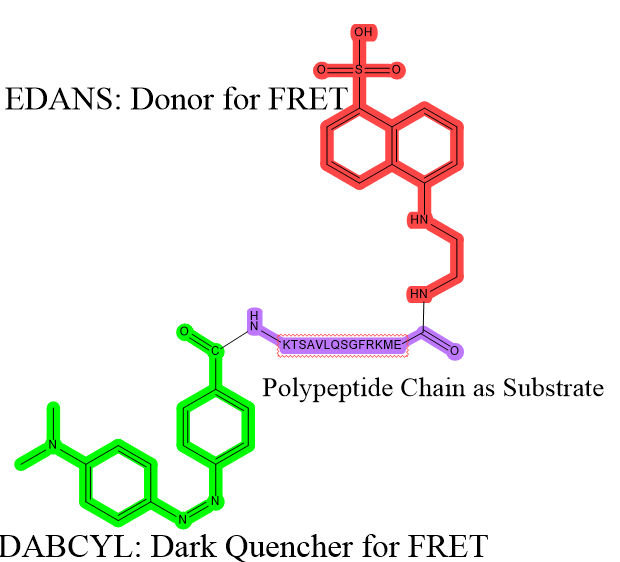
\includegraphics[width=0.5\linewidth]{../Figures/fluorescent substrate.png}
    \caption{Structure of Fluorescent Substrate}
    \label{Structure of Fluorescent Substrate}
\end{figure}

The overall consequence is that, when the substrate is consumed, then, it will show fluorescence.
Further process of reaction will lead to more intensive fluorescence which can be detected by \textbf{ELISA} in the unit of RFU.

\subsection{Methods}

The independent variable in Michaelis Menton Equation is the concentration of substrate $[S]$.
Thus to verify the equation we must configure the substrate solution of different concentrations.
We started by dissolving 2 mg solid substrate into 192 $\mu$L DMSO solvent, which has the concentration of 5000 $\mu$L.
Then, we adjusted the ratio of DMSO and concentrated substrate to achieve 8 different concentrations of substrate solution, as shown in Table \ref{Substrate Solution Configuration in Microplate}.

We detected the speed of reaction by the concentration variation of fluorescent substrate which was identified by \textbf{enzyme-linked immunosorbent assay (ELISA)}.
The original data is shown in Figure \ref{Reaction Rate versus Substrate Concentration: 8 groups of experiments}.

\subsection{Data Analysis}

The original data gotten from \textbf{ELISA} is visualized in Figure \ref{Reaction Rate versus Substrate Concentration: 8 groups of experiments}.
In each subfigure, I have drawn the three parallelled groups of same substrate concentration.
It should be noted that, the several initial points were omitted for keeping linear parts only in accordance with the assumptions of Michaelis Menton Equation (the [ES] has reached steady state, not changing with time).

I performed linear regression to each of them, then averaged the slope which represents the speed of reaction.

The eight slopes (speed of reaction) were plotted with respect to substrate concentration [S] then.
As shown in Figure \ref{Reaction Rate versus Substrate Concentration: in normal axes}, the consequence is a curve which was similar to the prediction of Michaelis Menton Equation.

To further analyze the results, however, I converted the axes to the reciprocal of speed $V_0^{-1}$ and substrate concentration $[S]^{-1}$.
The benefit of reciprocal plotting is that we can operate linear regression again.
$$
\frac{1}{V_0}=\frac{K_m}{V_{max}}\cdot \frac{1}{[S]}+\frac{1}{V_{max}}\\
$$
$$
y=kx+b
$$
The vertical intercept b is $\frac{1}{V_{max}}$ and the horizontal intercept corresponds to $-\frac{1}{K_m}$, which are also annotated in Figure \ref{Reaction Rate versus Substrate Concentration: in reciprocall axes}.

\begin{figure}
    \centering
    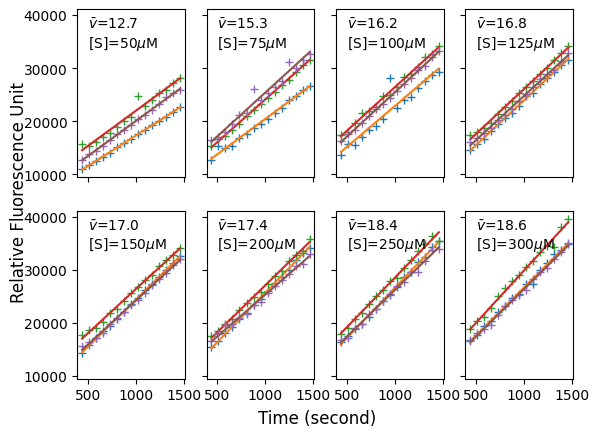
\includegraphics[width=1\linewidth]{../Figures/substrate1.png}
    \caption{Reaction Rate versus Substrate Concentration: 8 groups of experiments, each has 3 parallel groups}
    \label{Reaction Rate versus Substrate Concentration: 8 groups of experiments}
\end{figure}

\begin{figure}
    \centering
    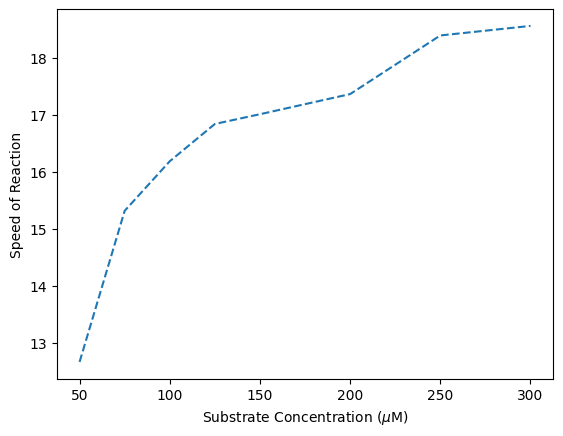
\includegraphics[width=1\linewidth]{../Figures/substrate2.png}
    \caption{Reaction Rate versus Substrate Concentration: in normal axes}
    \label{Reaction Rate versus Substrate Concentration: in normal axes}
\end{figure}

\begin{figure}
    \centering
    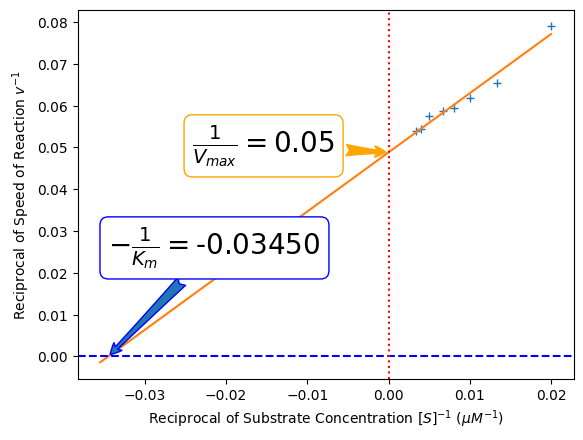
\includegraphics[width=1\linewidth]{../Figures/substrate3.png}
    \caption{Reaction Rate versus Substrate Concentration: in reciprocal axes}
    \label{Reaction Rate versus Substrate Concentration: in reciprocall axes}
\end{figure}


\section{Detecting Half-maximal Inhibitory Concentration}

\subsection{Principles}
\begin{figure}
    \centering
    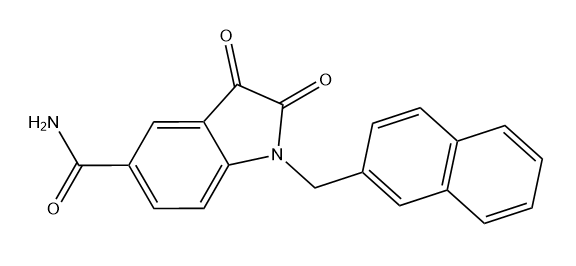
\includegraphics[width=0.7\linewidth]{../Figures/inhibitor structure.png}
    \caption{Structure of Inhibitor}
    \label{Structure of Inhibitor}
\end{figure}
The structure of inhibitor is shown in Figure \ref{Structure of Inhibitor}.
It will repress the reaction catalyzed by 3CL protease probably by competitive binding to the enzyme.
And we will determine the \textbf{Half-maximal Inhibitory Concentration, $IC_{50}$} through speed of reaction.
\subsection{Methods}
The inhibitor is consist of competitive inhibitor, uncompetitive inhibitor and mixed inhibitor.
Instead of changing substrate concentration simultaneously, we varied inhibitor concentration [I] only and keep [S] under control.
Also, we focused on \textbf{Half-maximal Inhibitory Concentration ($IC_{50}$)} only, without concerns about modified factors to $V_{max}$ or $K_m$.

The following procedure was used to prepare to inhibitor solution with different concentration:

% List
\begin{itemize}
    \item sample 20 $\mu$L concentrated inhibitor(20 mM) solution with 180 $\mu$L DMSO as additional solvent. Then mix in $1^{st}$ well of microplate, which has the concentration of 200 $\mu$M.
    \item prepare 30 $\mu$L DMSO in each well of $1^{st}$ raw.
    \item take 30 $\mu$L solution from $1^{st}$ to $2^{nd}$ and mix in $2^{nd}$ well.
    \item repeat the step for the following wells to perform two fold serial dilution as shown in Figure \ref{Serial Dilution of Inhibitor}.
\end{itemize}

To get the solution of substrate, we decanted 1.92 mL DMSO into 2 mg fluorescent substrate then separated it into twelve different wells in the same row.
As shown in Figure \ref{Inhibitor Solution Configuration in Microplate}, the substrate and inhibitor were in different rows.
To be noted that, in reality, they were also stored in separated microplates to avoid unwanted illumination of fluorescent substrate.



\subsection{Data Analysis}
The reaction speed was also detected by \textbf{ELISA}.
Twelve subfigures are shown in Figure \ref{Reaction Rate versus Inhibitor Concentration: 12 groups of experiments, each has 3 parallel groups} and each of them corresponds to a different inhibitor concentration [I].
There are two intriguing phenomena in the figure.
Firstly, one group in [I]=10 $\mu$M and one group in [I]=1.25 $\mu$L exist extreme fluctuations which may caused by bubbles in solution.
Secondly, the reaction speed has negative value in high concentration of inhibitor.
The major cause of that absurd phenomenon is probably the unsteady state with fluctuation at early initial period.
To eliminate the negative value and disturbance of it, I also decided to omit the early four points, which should reasonable and appropriate.

\begin{figure}
    \centering
    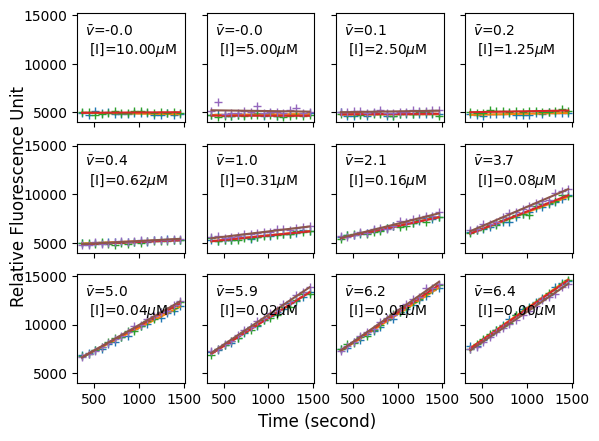
\includegraphics[width=1\linewidth]{../Figures/inhibitor1.png}
    \caption{Reaction Rate versus Inhibitor Concentration: 12 groups of experiments, each has 3
    parallel groups}
    \label{Reaction Rate versus Inhibitor Concentration: 12 groups of experiments, each has 3
    parallel groups}
\end{figure}

I performed linear regression again to each group and average the parallel groups to get the mean speed of reaction.
Then the plot of mean speed $\bar{V_0}$ versus inhibitor concentration was drawn.
From Figure \ref{Reaction Rate versus Inhibitor Concentration: determining IC50}, we can identify the \textbf{Half-maximal Inhibitory Concentration $IC_{50}$}, which is $IC_{50}=0.095\ \mu M$.

\begin{figure}
    \centering
    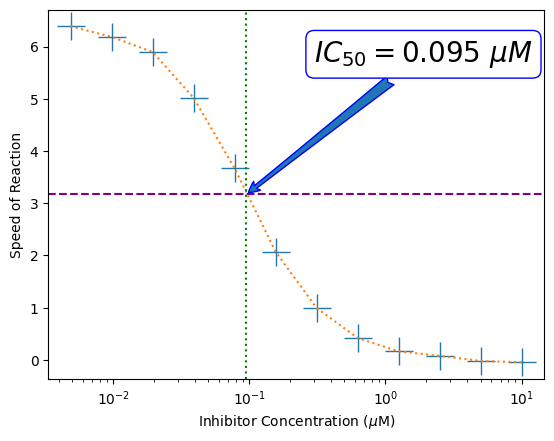
\includegraphics[width=1\linewidth]{../Figures/inhibitor2.png}
    \caption{Reaction Rate versus Inhibitor Concentration: determining IC50}
    \label{Reaction Rate versus Inhibitor Concentration: determining IC50}
\end{figure}



\bibliographystyle{plain}
\bibliography{references}
\end{document}